\documentclass{CUP-JNL-FMP}%


%%%% Packages
\usepackage{graphicx}
\usepackage{multicol,multirow}
\usepackage{amsmath,amssymb,amsfonts}
\usepackage{mathrsfs}
\usepackage{amsthm}
\usepackage{rotating}
\usepackage{appendix}
\usepackage[numbers]{natbib}
\usepackage{ifpdf}
\usepackage[T1]{fontenc}
\usepackage{newtxtext}
\usepackage{newtxmath}
\usepackage{textcomp}
\usepackage[colorlinks,allcolors=weblmcolor]{hyperref}

\newtheorem{theorem}{Theorem}[section]
\newtheorem{lemma}[theorem]{Lemma}
\theoremstyle{definition}
\newtheorem{remark}[theorem]{Remark}
\newtheorem{example}[theorem]{Example}
\numberwithin{equation}{section}


\articletype{RESEARCH ARTICLE}
%\artid{20}
\jyear{2021}
%\jvol{4}
%\jissue{1}
\jdoi{10.1017/fmp.2021.X}
%\raggedbottom


\begin{document}

\begin{Frontmatter}

\title[Hypersurfaces with Small Steklov Eigenvalues]{Hypersurfaces with Prescribed Boundary and Small Steklov Eigenvalues}

\author[1]{Bruno Colbois}\orcid{0000-0002-8514-4315}
\author[2]{Alexandre Girouard}\orcid{0000-0001-8823-831X}
\author[3]{Antoine M\'etras}\orcid{0000-0002-0251-345}

\authormark{Bruno Colbois \textit{et al}.}

\address[1]{\orgname{Universit\'e de Neuch\^atel, Institut de Math\'ematiques, Rue}, \orgaddress{\street{Rue Emile-Argand 11}, \postcode{CH-2000 Neuch\^atel}, \country{Switzerland}};\email{bruno.colbois@unine.ch}}
\address[2]{\orgdiv{D\'epartement de math\'ematiques et de 	statistique}, \orgname{Univer\-sit\'e Laval, Pavillon Alexandre\-Vachon}, \orgaddress{\street{1045, av. de la M\'edecine}, \city{Qu\'ebec}, \postcode{Qc G1V 0A6}, \country{Canada}};\email{alexandre.girouard@mat.ulaval.ca}}
\address[3]{\orgdiv{D\'epartement de math\'ematiques et de statistique}, \orgname{Universit\'e de Montr\'eal}, \orgaddress{\street{CP 6128 succ Centre-Ville}, \city{Montr\'eal}, \postcode{QC H3C 3J7}, \country{Canada}}; \email{metrasa@dms.umontreal.ca}}


\received{04 May 2020}
%\revised{10 May 2020}
\accepted{12 May 2020}

\keywords{Steklov eigenvalues, hypersurfaces}

\keywords[MSC Codes]{\codes[Primary]{35P15}; \codes[Secondary]{58C40, 53A07}}


\abstract{Given a smooth compact hypersurface $M$ with boundary $\Sigma=\partial M$, we prove the existence of a sequence $M_j$ of hypersurfaces with the same boundary as $M$, such that each Steklov eigenvalue $\sigma_k(M_j)$ tends to zero as $j$ tends to infinity. The hypersurfaces $M_j$ are obtained from $M$ by a local perturbation near a point of its boundary. Their volumes and diameters are arbitrarily close to those of $M$, while the principal curvatures of the boundary remain unchanged.}

\end{Frontmatter}

\localtableofcontents

\vspace*{14pt}
\section{Introduction}
Let $M$ be an $n$-dimensional smooth compact Riemannian manifold with boundary $\Sigma=\partial M$.  The Steklov
eigenvalue problem on $M$ consists in\vadjust{\clearpage} finding all numbers $\sigma\in\mathbb{R}$ for which there exists a nonzero function $u \in C^\infty(M)$, which solves
\begin{equation*}
    \begin{cases}
        \Delta u = 0 & \text{in  $M$,} \\
        \partial_\nu u = \sigma u & \text{on  $\Sigma$.}
    \end{cases}\vspace*{-2pt}
\end{equation*}
Here, $\Delta$ is the Laplacian induced from the Riemannian metric $g$ on $M$, and $\partial_\nu$
is the outward pointing normal derivative along the boundary $\Sigma$. The Steklov eigenvalues
form an unbounded increasing sequence
$0 = \sigma_0 \leq \sigma_1 \leq \sigma_2 \leq \dots \to \infty$, each of which is repeated according to its multiplicity.
Note that if $M$ is connected, then $\sigma_1>0$.
See \cite{GP17,legacy} for background on this problem.

\looseness-1One of our main interests in recent years has been to understand the particular role that the boundary  $\Sigma$ plays with respect to Steklov eigenvalues. Some papers studying this question are \cite{CGH18, PS16,CESG17,CG18,WX09,Kar15,GPPS,CGG17,shamma}.
In particular, we have considered the effect of various geometric constraints on individual eigenvalues $\sigma_k$. One particularly interesting question is to prescribe a Riemannian metric $g_\Sigma$ on the boundary $\Sigma$ and to investigate lower and upper bounds for the eigenvalue $\sigma_k$ among all Riemmanian metrics $g$ that coincide with $g_\Sigma$ on the boundary. Given any Riemannian metric $g$ on $M$ such that $g=g_\Sigma$ on $\Sigma$, it is proved in \cite{CESG17} that one can make any eigenvalue $\sigma_k$ arbitrarily small by modifying the Riemannian metric $g$ in an arbitrarily small neighborhood $V\subset M$ of a point $p\in\partial M$. More precisely, for each $\epsilon>0$ and each $k\in\mathbb{N}$, there exists a Riemannian metric $\widetilde{g}=\widetilde{g}_{\epsilon,k}$ on $M$ that coincides with $g_\Sigma$ on $\Sigma$ and also with $g$ outside the neighborhood $V$, such that $\sigma_k(M,\widetilde{g})<\epsilon$. For manifolds $M$ of dimension $n\geq 3$, one can also obtain arbitrarily large eigenvalues, but in general not using a perturbation that is localized near the boundary of $M$ (see \cite{CESG17,CG18}). In \cite{CGG17} a more restrictive constraint was imposed by requiring the manifold $M$ to be a submanifold of $\mathbb{R}^m$ with prescribed boundary $\Sigma=\partial M\subset\mathbb{R}^m$. In this context an upper bound for $\sigma_k$ was given in terms of $\Sigma$ and of the volume of $M$. The authors were unable at the time to give a lower bound and they raised the question of whether one exists, or if instead, arbitrarily small eigenvalues are possible. The goal of this paper is to answer that question.

\begin{theorem}\label{thm:main}
Let $M \subset \mathbb{R}^{n+1}$ be a smooth $n$-dimensional compact hypersurface with nonempty boundary $\Sigma=\partial M$. For each $p \in \Sigma$, there exists a sequence of hypersurfaces $M_j\subset\mathbb{R}^{n+1}$, $j\in\mathbb{N}$, with boundary $\partial M_j=\Sigma$
% Remarque 2
and with the hypersurface $M_j$ coinciding with $M$ outside of a ball $B(p, \frac{1}{j})$,
such that\vspace*{-2pt}%
\begin{gather}\label{limit:mainthm}
\lim_{j\to\infty}\sigma_k(M_j)=0\qquad\mbox{ for each }k\in\mathbb{N}.
\vspace*{-2pt}%
\end{gather}
% The hypersurface $M_j$ coincides with $M$ outside of a ball $B(p,\frac{1}{j})$ and
The principal curvatures of $\Sigma\subset M_j$ are independent of $j$. Moreover,
the volume and diameter of $M_j$ converge to those of $M$ as $j\to\infty$.
\end{theorem}

In order for \eqref{limit:mainthm} to hold for each $k\in\mathbb{N}$, it is necessary that the perturbed hypersurfaces $M_j$ differ from $M$ arbitrarily close to the boundary $\Sigma$ as $j\to\infty$. Indeed, let $b$ be the number of connected components of $\Sigma$ and note that any hypersurface $\widetilde{M}$ that coincides with $M$ in a neighborhood $\Omega$ of $\Sigma$ satisfies
$\sigma_{b+1}\geq C>0$, where $C$ is given by a sloshing problem on $\Omega\cap M$; see \cite{CGG17} for details.

\begin{remark}\label{remark:regularitycodim}
 Theorem \ref{thm:main} holds in arbitrary positive codimension and ambient space. We decided to state it for hypersurfaces in $\mathbb{R}^{n+1}$for the sake of notational simplicity. Note also that Theorem~\ref{thm:main} certainly holds under weaker regularity asumptions.
\end{remark}

\begin{remark}\label{remark:noncommutative}
By construction (see Section \ref{section:perturbation}), each manifold $M_j$ coincides with $M$ in a neighborhood $\Omega_j$ of its prescribed boundary $\Sigma$.
  Hence, the Dirichlet-to-Neumann maps $D_j\colon C^\infty(\Sigma)\rightarrow C^\infty(\Sigma)$ associated with $M_j$ all have the same full symbol~\cite{LeeUhlmann}.
  The asymptotic behavior of $\sigma_k(M_j)$ as $k\to\infty$ is therefore independent of $j$. That is, for each $j_1, j_2\in\mathbb{N}$ the following holds:
    $\sigma_k(M_{j_1})-\sigma_k(M_{j_2})=O(k^{-\infty})$; see~\cite[Lemma 2.1]{GPPS}. In particular, the limits of $\sigma_k(M_j)$ as $j\to\infty$ and as $k\to\infty$ do not commute.
\end{remark}

\vspace*{-10pt}%
\subsection{The Strategy of the Proof}
For eigenvalues of the Laplace operator, it is well known that one can obtain arbitrarily small eigenvalues by constructing thin Cheeger dumbbells in the interior of the manifold; see \cite{Chavel,CoursColboisMtl}. This strategy does not work for Steklov eigenvalues. For Steklov eigenvalues, it is possible to obtain arbitrarily small eigenvalues by creating thin channels, but this involves deformation of the boundary or a perturbation of the Riemannian metric in the interior of $M$; see \cite{GP10,CESG17}. In order to prove Theorem \ref{thm:main}, we have to use a more elaborate strategy.

Given a smooth function $\widetilde{u}\colon \mathbb{R}^{n+1}\rightarrow\mathbb{R}$, consider the restriction $u=\widetilde{u}\bigl|\bigr._{{M}}$.
It is well known that if $\int_{\Sigma}u\,dA=0$,
\begin{gather}\label{ineq:variationalintro}
\sigma_1(M)\int_{\Sigma}u^2\,dA\leq\int_M|\nabla u|^2\,dV;
\end{gather}
see \cite{GP17} and Section \ref{section:prelim} below. Here $\nabla u$ is the tangential gradient of $u$. It is the projection of the ambient gradient $\overline{\nabla}\widetilde{u}$ on the tangent spaces of $M\subset\mathbb{R}^{n+1}$. The basic idea of our proof is to fix a function $\widetilde{u}\in C^\infty(\mathbb{R}^{n+1})$ and consider the vector field $\overline{\nabla}\widetilde{u}$ in the ambient space $\mathbb{R}^{n+1}$. The hypersurface $M$ is then deformed by creating ``wrinkles''  that tend to make the various tangent spaces $T_pM$, for $p\in\mbox{int }M$, perpendicular to $\overline{\nabla}\widetilde{u}(p)$. This is achieved by ``folding the surface like an accordion'' in the direction perpendicular to $\overline{\nabla}\widetilde{u}$. In the limit the right-hand-side of inequality \eqref{ineq:variationalintro} tends to zero.
Let us illustrate this strategy with a simple example.

\begin{example}
Given a smooth function $f\colon \overline{\mathbb{D}}\rightarrow\mathbb{R}$ vanishing on the circle $S^1=\partial\mathbb{D}$, consider the surface
$$
S_f:=\mbox{Graph of }f=
\big\{(x,y,f(x,y)) : (x,y)\in\overline{\mathbb{D}}\big\}.
$$
The boundary of $S_f$ is the same for each $f$.
We will use the function defined by $\widetilde{u}(x,y,z)=x$ and its restriction $u=\widetilde{u}|_{S_f}$ as a trial function in inequality \eqref{ineq:variationalintro}. Because $\nabla\widetilde{u}=(1,0,0)$, it follows from Lemma~\ref{lemma:dirichletgraph} that the Dirichlet energy of $u:=\widetilde{u}
\bigl|\bigr._{{S_f}} \colon S_f\rightarrow\mathbb{R}$ is given by
$$\int_{S_f}|\nabla u|^2=\int_{\mathbb{D}} \frac{1 + f_y^2}{\sqrt{1 + f_x^2+f_y^2}}
\,dxdy.$$
For $n\in\mathbb{N}$, define $f=f_n\colon \overline{\mathbb{D}}\rightarrow\mathbb{R}$ by
$$f(x,y)=\sin(nx)(\overbrace{1-x^2-y^2}^{\phi(x,y)}).$$
It follows from
\begin{gather*}
f_x^2=n^2\Bigl(\cos(nx)\phi+\frac{1}{n}\sin(nx)\phi_x\Bigr)^2\quad\mbox{ and }\quad
f_y^2=\sin^2(nx)\phi_y^2
\end{gather*}
that
$$\lim_{n\to\infty}\int_{S_{f_n}}|\nabla u|^2=0.$$
Together with \eqref{ineq:variationalintro}, this shows that
$\lim_{n\to\infty}\sigma_1(S_{f_n})=0.$
\end{example}


The proof of Theorem \ref{thm:main} is based on the above idea, but it is technically more involved, because we want to localize this argument to a small neighbourhood of a point $p$ of the boundary. This is a significant gain compared to the above example, because it allows the construction of an arbitrary finite number of disjointly supported trial functions with small Dirichlet energy, leading to the collapse of each eigenvalue $\sigma_k$ rather than just $\sigma_1$. For the sake of readability and simplicity, the deformations that we use in the proof of Theorem \ref{thm:main} are Lipschitz continuous but only piecewise smooth. This is not problematic because only integrals of the first derivatives of these deformations appear.


\subsection*{Plan of the Paper}
In Section \ref{section:prelim} we review the min-max characterization of Steklov eigenvalues, and we prove a lemma regarding the control of the Dirichlet energy under quasi-isometries. We then proceed to construct the perturbed hypersurfaces in Section \ref{section:perturbation}. We use a quasi-isometric chart to a hypersurface with a flat boundary. The perturbed submanifold is then constructed by considering the graph
of a locally supported oscillating function. Finally, in Section \ref{section:testfunction} an appropriate trial function is used to conclude the proof of Theorem \ref{thm:main}.


\section{Notation and Preliminary Considerations}\label{section:prelim}

Let $M$ be a smooth compact manifold with boundary $\Sigma$. The volume form on $M$ is written $dV$, while
the volume form on $\Sigma$ is $dA$. We denote by $H^1(M)$ the standard Sobolev space of functions in $ L^2(M,dV)$ with weak first derivative in $L^2(M,dV)$.
The Steklov eigenvalues $\sigma_k$ admits a variational characterization in terms of the \emph{Steklov--Rayleigh quotient} of a function $0\neq u \in H^1(M)$,
\begin{equation*}\label{StekRayleighQuotient}
    \mathcal{R}(u) = \frac{\int_{M} |\nabla u|^2\,dV}{\int_{\Sigma} u^2\,dA}.
\end{equation*}
The numerator $D(u)=\int_{M} |\nabla u|^2\,dV$ is the \emph{Dirichet energy} of $u\in H^1(M)$.
It is well known that
\begin{equation}\label{eq:minmaxsigmak}
    \sigma_k = \min_{\substack{S \subset H^1(M) \\ \dim S = k+1}}
    \max_{u \in S \setminus \{0\}} \mathcal{R}(u),
\end{equation}
where the minimum is taken over all $(k+1)$-dimensional linear subspaces $S\subset H^1(M)$.

\subsection{Quasi-isometries and Dirichlet Energy}

Let $M$ and $\widetilde{M}$ be two $n$-dimensional Riemannian manifolds with boundary. A diffeomorphism $\phi\colon M\rightarrow\smash{\widetilde{M}}$ is a \emph{quasi-isometry} with constant $C\geq 1$ if for each $p\in M$ and each $0\neq v\in T_pM$,
$$\frac{1}{C}\leq\frac{\|D_p\phi(v)\|^2}{\|v\|^2}\leq C.$$
Quasi-isometries provide a control of the Dirichlet energy of a function.
\begin{lemma}\label{lemma:QIcontrolEnergy}
Let $\phi\colon M\rightarrow\widetilde{M}$ be a quasi-isometry with constant $C\geq 1$. Let $f\in H^1(\widetilde{M})$; then
$$\frac{1}{C^{\frac{n}{2}+1}}\leq\frac{\|\nabla (f\circ\phi)\|_{L^2(M)}^2}{\|\nabla f\|_{L^2(\widetilde{M})}^2}\leq C^{\frac{n}{2}+1}.$$
\end{lemma}
\begin{proof}
Let $\widetilde{g}$ be the Riemannian metric of $\widetilde{M}$ and let $g$ be that of $M$. Let $\widehat{g}=\phi^\star(\widetilde{g})$ be the pull-back of the metric $\widetilde{g}$. Because $\phi$ is a quasi-isometry with constant $C$, the following holds for each $0\neq v\in TM$,
$$\frac{1}{C}\leq \frac{g(v,v)}{\widehat{g}(v,v)}\leq C.$$
It follows that
$$\frac{1}{C}g(\nabla_{g}f,\nabla_{g}f)\leq\widehat{g}(\nabla_{\widehat{g}}f,\nabla_{\widehat{g}}f)\leq Cg(\nabla_{g}f,\nabla_{g}f).$$
The corresponding volume forms satisfy
$$C^{-n/2}dV_g\leq dV_{\widehat{g}}\leq C^{n/2}dV_g.$$
This leads to
\begin{align*}
\|\nabla (f\circ\phi)\|_{L^2}^2&=\int_M g\bigl(\nabla_g (f\circ\phi),\nabla_g(f\circ\phi)\bigr)\,dV_g\\
&\leq
C^{n/2+1}\int_M {\widehat{g}}\bigl(\nabla_{\widehat{g}} (f\circ\phi),\nabla_{\widehat{g}} (f\circ\phi)\bigr)\,dV_{\widehat{g}}\\
&=
C^{n/2+1}\int_{\widetilde{M}} {\widetilde{g}}(\nabla_{\widetilde{g}} f,\nabla_{\widetilde{g}} f)\,dV_{\widetilde{g}}.
\end{align*}
The proof of the lower bound is identical, and accordingly omitted.
\end{proof}

\subsection{Quasi-isometric Charts}
Recall that a subset $M\subset\mathbb{R}^{n+1}$ is a hypersurface with boundary if for each $p\in M$, there exist open sets $W,W'\subset\mathbb{R}^{n+1}$ with $p\in W$ and a diffeomorphism $\psi:W\rightarrow W'$ such that
$\psi(M\cap W)$ is an open set in the half-space
$$H=\{x\in\mathbb{R}^{n+1} : x_{n+1}=0, x_1\geq 0\}.$$
The point $p\in M$ is on the boundary $\Sigma$ of $M$ if and only if $\psi$ sends it to the boundary of the \nobreak{half-space}~$H$:
$$\psi(p)\in\partial H:=\{x\in H : x_1=0\}.$$
This definition is coherent. It does not depend on the choice of the diffeomorphism $\psi$;
see \cite[Chapter~1]{Hi76} for details.
By further restricting $\psi$ and scaling if necessary, we can assume that it is a quasi-isometry and that its image $W'$ is a cylinder.
This is summed up in the next lemma.
\begin{lemma}\label{lemma:flatchart}
	For each $p\in\Sigma$, there exists a quasi-isometry
	$$\psi\colon W\longrightarrow W'=B_{\mathbb{R}^n}(0,1)\times (-1,1)$$
	with $\psi(p)=0$ and such that the image of $M\cap W$ is
	$$U:=\psi(M\cap W)=\{x\in H : |x|<1\}.$$
\end{lemma}
\begin{remark}
	We identify $U\subset\mathbb{R}^{n+1}$ with a subset of $\mathbb{R}^n$ so that we can write $x=(x_1,\dots,x_n)\in U$ instead of
	$x=(x_1,\dots,x_n,0)\in U$.
\end{remark}
\begin{figure}[h]
\FIG{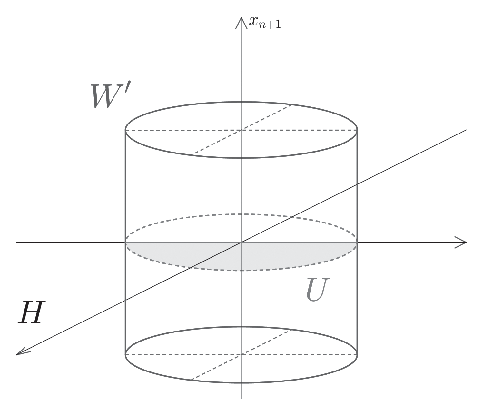
\includegraphics{Fig1.eps}}
{\caption{The domain $U$}}
\end{figure}
In particular, the restriction of $\psi$ to $\Sigma\cap W$ is also a quasi-isometry.

\subsection{Dirichlet Energy on the Graph of a Function}
Let $U\subset\mathbb{R}^n$ be a bounded open set and let $f\colon U\rightarrow\mathbb{R}$ be a bounded smooth function. Consider the graph
$$S_f=\{(x,f(x)) : x\in U\}\subset\mathbb{R}^{n+1}.$$
Given a function $u\colon U\rightarrow\mathbb{R}$, define $\widetilde{u}\colon U\times\mathbb{R}\rightarrow\mathbb{R}$ by $\widetilde{u}(x,x_{n+1})=u(x)$ and define $u_f\colon S_f\rightarrow\mathbb{R}$ by
\begin{gather}\label{defuf}
  u_f(x,f(x)) = u(x)=\widetilde{u}\bigl|\bigr._{{S_f}}.
\end{gather}

\begin{lemma}\label{lemma:dirichletgraph}
	The Dirichlet energy of $u_f\colon S_f\rightarrow\mathbb{R}$ is
	\begin{equation}\label{eq:dirichletgraph}
	\int_{S_f} |\nabla u_f|^2\,dV
	= \int_U \frac{|\nabla u|^2 + |\nabla u|^2 |\nabla f|^2
	-\langle {\nabla u}, {\nabla f} \rangle^2}{\sqrt{1 + |\nabla f|^2}}
	\,dx,
	\end{equation}
	where on the left-hand-side $\nabla$, $dV$, and the norm are taken on $S_f$, and on the right-hand-side $dx=dx^1\cdots dx^n$ is the Lebesgue measure on $U$, while $\nabla$ is the usual gradient on $\mathbb{R}^n$.
\end{lemma}

	The Cauchy--Schwarz inequality gives $|\nabla u|^2 |\nabla f|^2
- \langle {\nabla u}, {\nabla f} \rangle^2 \geq 0$ with equality if and only
if $\nabla u = c \nabla f$ for some constant $c$.

\begin{proof}[Proof of Lemma \ref{lemma:dirichletgraph}]
	To simplify notation, we will write $S=S_f$.
	For any point $p\in S$, the gradient $\nabla u_f\in T_pS$ is the projection of $\overline{\nabla}\widetilde{u}$ on $T_pS$,
	that is,
	\begin{equation*}
	\nabla u_f = \overline{\nabla} \widetilde{u} -
\langle {\overline{\nabla} \widetilde{u}}, {N} \rangle N,
	\end{equation*}
	where $N$ is a unit normal vector to $T_pS$.
	It follows from
	\begin{align*}
	\nabla\widetilde{u} &= \Big(\frac{\partial u}{\partial x_1}, \dots, \frac{\partial u}
	{\partial x_n}, 0\Big),
	\\%\end{equation*}
	%and
	%\begin{equation}
	N &=\frac{1}{\sqrt{1 + |\nabla f|^2}}\Big(e_{n+1}-\sum_{i=1}^n\frac{\partial f}{\partial x_i}e_i\Big).
	\end{align*}
	that
	\begin{gather}\label{identity:nablauf}
	|\nabla u_f|^2
	= \frac{|\nabla u|^2 + |\nabla u|^2|\nabla f|^2
		- \langle {\nabla u}, {\nabla f} \rangle^2}{1 + |\nabla f|^2}.
	\end{gather}
	
	The volume element on $S_f$ is given by
	\begin{equation}
	dV %= \frac{1}{\sqrt{1 + |\nabla f|^2}}(1 + |\nabla f|^2)
	= \sqrt{1 + |\nabla f|^2}.
	\end{equation}
	Together with identity \eqref{identity:nablauf}, this completes the proof.
\end{proof}


\section{Perturbation of the Submanifold $M$}\label{section:perturbation}

Given $p\in\Sigma$, let $\psi$ be the quasi-isometric chart provided by Lemma \ref{lemma:flatchart}. In order to prove Theorem \ref{thm:main}, we will deform the submanifold $M$ in the neighborhood $W$ of the point $p$ by deforming the neighborhood $U\subset W'$ inside $W'$ and pulling back to $W$ using the quasi-isometry $\psi$.
Consider a smooth function $f\colon U\rightarrow\mathbb{R}$ that is supported in the interior of $U$ and which satisfies $|f(x)|<1$ for each $x\in U$. This last condition implies that the graph of $f$,
$$S_f = \{(x, f(x)) : x\in U\},
$$
is contained in the cylinder $W'$.
Hence it can be used to define a deformation of $M$ as follows:
\begin{gather}\label{def:TM}
\widetilde{M}_f:=(M\setminus W)\cup\psi^{-1}(S_f).
\end{gather}
Because $f$ is smooth and supported in $U$ and $S_f\subset W'$, the subset $\widetilde{M}_f\subset\mathbb{R}^{n+1}$ is also  a submanifold with boundary $\partial\widetilde{M}_f=\Sigma=\partial M$.
  \begin{remark}
    It might be possible to prove Theorem~\ref{thm:main} by performing a deformation of $M$ directly in the ambient space $\mathbb{R}^{n+1}$, but it appears to be simpler to use quasi-isometric charts.
  \end{remark}


\subsection{Deformation Function}

We now construct specific functions $f$ and $u$ such that the Dirichlet energy of $u_f$, defined by~\eqref{defuf}, is small. Our method is based on Lemma~\ref{lemma:dirichletgraph}, which shows that if $\nabla u$ and $\nabla f$ are parallel the numerator of~\eqref{eq:dirichletgraph} is independent of $\nabla f$, while the denominator behaves as $|\nabla f|$. Thus, we want $f$ and $u$
to have parallel gradients with $|\nabla f|$ big to get a small Dirichlet
energy for $u_f$.

Consider numbers
$\epsilon, \partial_1, \partial_2, \rho > 0$ that are sufficiently small and define
$\partial:=\partial_1 + \partial_2$. These constants will be adjusted later in equation \eqref{dfn:constants}.
Let $q = (\partial, 0, \dots, 0)\in H$. Consider the following subsets of $U$:
\begin{align*}
  A &:= \big\{(x_1, \dots, x_n) \mid  x_1 \geq \partial, \|x - q\| \leq \epsilon\big\}, \\
  B &:= \big\{(x_1, \dots, x_n) \mid  \partial_1 \leq x_1 \leq \partial,
      \|\Pi x\| \leq \epsilon\big\}, \\
  C &:= \big\{(x_1, \dots, x_n) \mid  0 \leq x_1 \leq \partial_1,
      \|\Pi x\| \leq \epsilon\big\}, \\
  D &:= \big\{x \in U \setminus (A \cup B \cup C) \mid  d(x,A \cup B \cup C),
      \leq \rho\big\}
\end{align*}
where $\Pi(x_1, x_2, \dots, x_n) = (x_2, \dots, x_n)$ is the projection
on the boundary. Let $\Omega = A \cup B \cup C$. See Figure \ref{fig:domain}, where the $x_1$-axis is vertical.
\begin{figure}[h]
\FIG{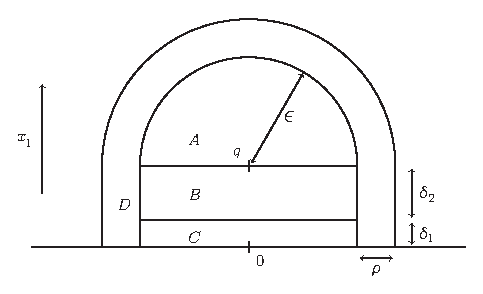
\includegraphics{Fig2}}
{\caption{Perturbation region}\label{fig:domain}}
\end{figure}

Define cutoff functions
\begin{align*}
  \eta &\colon  [0, \infty) \to \mathbb{R}, & \gamma &\colon  [0, \partial]  \to \mathbb{R}, \\
  \eta(t) &= \max\{0, 1- t\}, &
  \gamma(t) &=
  \begin{cases}
    0 & \text{if $t \leq \partial_1$,} \\
    t - \partial_1 & \text{if $\partial_1 \leq t \leq \partial$}.
  \end{cases}
\end{align*}
Finally, define $F \colon  [0, \infty) \to \mathbb{R}$ to be periodic
of period 4, given on the interval $[0,4]$ by
\begin{align*}
  F(t) = \begin{cases}
    1 - t & \text{if $t \in [0,2]$,}\\
    t - 3 & \text{if  $t \in [2,4]$}.
  \end{cases}
\end{align*}
Given $\omega>0$, define $f \colon  U \rightarrow \mathbb{R}$ by
\begin{equation}\label{eq:deffx}
  f(x) =
  \begin{cases}
    \eta\big(\frac{d(x,\Omega)}{\rho}\big)
    \gamma(x_1) F(\omega \|\Pi x\|) &
    \text{if $x_1 \leq \partial$,} \\
    \eta\big(\frac{d(x, \Omega)}{\rho}\big)
    \partial_2 F(\omega \|x - q \|) & \text{if $x_1 \geq \partial$.}
  \end{cases}
\end{equation}
Note that functions $\eta$ and $\gamma$ are used to localize the deformation function $f$.
% Remarque 4
In particular, the use of the function $\gamma$ restrict the deformation function $f$ outside a neighborhood of the boundary,
hence keeping this neighborhood fixed under the deformation.
The parameter $\omega$ will be sent to $\infty$ later in the proof.
It is important to remark that $|F'(x)| = 1$ at points where
$F$ is differentiable and $|F(x)| \leq 1$ for all $x$.
\begin{remark}\label{rem:smoothing}
The deformation function $f$ is Lipschitz continuous and piecewise smooth. Because only integrals of first order derivatives of this function appear in the estimates below, one could replace it by smooth approximations without affecting the results.
\end{remark}

\section{Trial Function}\label{section:testfunction}

The trial function $u$ is supported on $\Omega\subset U$
and is defined by
\begin{equation}
  u(x) =
  \begin{cases}
    1 - \frac{\|\Pi x\|}{\epsilon} &\text{if $x \in B \cup C$,} \\
    1 - \frac{\|x - q\|}{\epsilon} &\text{if $x \in A$,}\\
    0 &\text{elsewhere}.
  \end{cases}
\end{equation}
By construction, the function $u_f$ defined by~\eqref{defuf} belongs to $H^1(S_f)$, and we can estimate its Dirichlet energy.
On $A$, the Dirichlet energy of $u_f$ can be made small by taking
$\omega$ big. Indeed, for almost all $x \in A$,
\begin{align}\label{eq:nablafonA}
  \nabla f &=
  \pm \partial_2 \omega \frac{x - q}{\|x - q\|}
  ,
  \\
  \nabla u &= -
  \frac{1}{\epsilon}\frac{x - q}{\|x - q\|}
  ,
\end{align}
and using the fact that $\nabla f$ and $\nabla u$ are parallel,
the Dirichlet energy is
\begin{align*}
  \int_{S_f \cap A \times \mathbb{R}} |\nabla u_f|^2 dV
  &= \int_A \frac{|\nabla u|^2}{\sqrt{1 + |\nabla f|^2}}\,dx
  = \frac{1}{\epsilon^2}
  \frac{1}{\sqrt{1 + \partial_2^2 \omega^2}} \mathop{\mbox{Vol}} A\\
  &= \frac{c_1 \epsilon^{n-2}}{\sqrt{1 + \partial_2^2 \omega^2}}
\end{align*}
where $c_1$ is some dimensional constant.

On $B$ and $C$, $\nabla f$ and $\nabla u$ are not parallel, but
it is possible to make the Dirichlet energy small by making
the volume of $B$ and $C$ small.
For $B$, we have for almost all $x \in B$:
\begin{align}\label{eq:nablafonB}
  \nabla f(x) &= F(\omega \|\Pi x\|) e_1 \pm \gamma(x_1) \omega
                \frac{\Pi x}{\|\Pi x\|}, \\
  \nabla u(x) &= -\frac{1}{\epsilon} \frac{\Pi x}{\|\Pi x\|},
\end{align}
and since $e_1$ and $\Pi x$ are orthogonal,
\begin{equation*}
  |\nabla f(x)|^2 = F(\omega \|\Pi x\|)^2 + \gamma(x_1)^2 \omega^2.
\end{equation*}
Then the Dirichlet energy on $B$ is
\begin{align*}
  \int_{S_f \cap B \times \mathbb{R}} |\nabla u_f|^2 dV
  &= \int_B \frac{\frac{1}{\epsilon^2} + \frac{1}{\epsilon^2}
    F(\omega \|\Pi x\|)^2}
    {\sqrt{1 + F(\omega \|\Pi x\|)^2 + \gamma(x_1)^2 \omega^2}}
    dx\\
  &\leq \frac{1}{\epsilon^2}
    \int_B \frac{2}{\sqrt{1 + \gamma(x_1)^2 \omega^2}} dx \\
  &= c_2 \epsilon^{n-3}
    \int_0^{\partial_2} \frac{1}{\sqrt{1 + x_1^2 \omega^2}} dx_1 \\
  &= c_2 \epsilon^{n-3}
    \frac{\ln(\partial_2 \omega + \sqrt{1 + \partial_2^2})}{\omega},
\end{align*}
where $c_2$ is a constant that depends only on the dimension.
And on $C$, since $f=0$, the Dirichlet energy is simply
\begin{equation*}
  \int_{S_f \cap C \times \mathbb{R}} |\nabla u_f|^2 dV = \frac{1}{\epsilon^2} \mathop{\mbox{Vol}} C
  = c_3 \partial_1 \epsilon^{n-3},
\end{equation*}
where $c_3$ is a constant that depends only on the dimension.
The denominator in the Steklov--Rayleigh quotient of $u_f$ satisfies
 $$\int_{B(0,\epsilon)}\Big(1-\frac{|x|}{\epsilon}\Big)^2\,dx\geq\frac{1}{4}\mathop{\mbox{Vol}}
 \Big({B\Big(0,\frac{\epsilon}{2}\Big)}\Big)=c_4\epsilon^{n-1},$$
for some constant $c_4>0$.
In total, the Steklov--Rayleigh quotient of $u_f$ on $S_f$ is bounded as follows:
\begin{align*}
  \mathcal{R}(u_f)
  &\leq \frac{1}{c_4\epsilon^{n-1}}
    \Big(c_1 \frac{\epsilon^{n-2}}{\sqrt{1 + \partial_2^2 \omega^2}}
    + c_2 \frac{\epsilon^{n-3} \ln(\partial_2 \omega +
    \sqrt{1 + \partial_2^2 \omega^2})}{\omega}
    + c_3 \partial_1 \epsilon^{n-3} \Big)\\
  &= \frac{1}{c_4}\Big(c_1 \frac{\epsilon^{-1}}{\sqrt{1 + \partial_2^2 \omega^2}}
    + c_2 \frac{\epsilon^{-2} \ln(\partial_2 \omega + \sqrt{1 +
    \partial_2^2 \omega^2})}{\omega}
    + c_3 \partial_1 \epsilon^{-2}\Big).
\end{align*}
We are now ready to define the constants more precisely. By using the following:
\begin{equation}\label{dfn:constants}
\partial_1 = \epsilon^3,\quad \partial_2 = \epsilon^{3/2},\quad \omega = \epsilon^{-3},\quad \rho=\epsilon,
\end{equation}
we obtain
\begin{equation*}
  \mathcal{R}(u_f) = \mathcal{O}(\epsilon^{1/2}) \quad \text{as } \epsilon \longrightarrow 0.
\end{equation*}
We have proved that a local perturbation of $U$ allows the construction
of a local trial function with arbitrarily small Steklov--Rayleigh quotient. The proof of our main result is now an easy consequence.
\begin{proof}[Proof of Theorem \ref{thm:main}]
  Without loss of generality, we work under the asumption that $k\in\mathbb{N}$ is fixed. The general case will then follow by a standard diagonal selection argument.
  Let $k,j \in \mathbb{N}$ with $j$ sufficiently large. Let $p_1, \dots, p_{k+1} \in B(p, \frac{1}{j}) \cap \Sigma$ be distinct points,
  and let $\psi$ be the quasi-isometric chart from Lemma \ref{lemma:flatchart}.
  For each $p_i$, we follow the above construction to obtain  deformation functions $f_i$ that are disjointly supported, by taking $\epsilon>0$ small enough, and trial functions $u_i$ that have disjoint supports contained in
    in $\psi(B(p,\frac{1}{j}) \cap M)$.
  By possibly choosing a smaller $\epsilon$ in the previous construction, we guarantee that the Rayleigh quotient of each $u_i$ is smaller than $1/j$.
     Consider the deformation function $f = f_1 + \dots + f_{k+1}$ supported in $B(p, {1}/{j})$ and the perturbed manifold $M_j = \smash{\widetilde{M}_f}$.
  Taking the pullback by $\psi$, we obtain $k+1$ trial functions $\psi^*(u_i)$ with disjoint supports and
  from Lemma \ref{lemma:QIcontrolEnergy}, their
  Rayleigh quotient is less than ${c}/{j}$ where $c$ is a constant depending on $\psi$.
  By the variational characterization \eqref{eq:minmaxsigmak} of the eigenvalue $\sigma_k$, we conclude that $\sigma_k(M_j) \leq {c}/{j}$.


  It remains to prove that the perturbed manifolds $M_j$ satisfy the geometric conditions from the theorem.
  Without loss of generality, we consider a single perturbation region $\Omega\cup D$ near one of the points $p_i$.
 Let $x \in \Omega$. There exists $x' \in \Omega$ such that
$f(x') = 0$, and the distance in $M_f$ between $x$ and $x'$ is
$\mathcal{O}(\epsilon^{3/2})$.
There is a path from $x'$
to some point $y$ on $\partial M$ such that the length of the path is less
than $\partial + \epsilon\pi/2 $, it suffices to
take the shortest path in $\{x \in M \mid  f(x) = 0\}$ from
$x'$ to $\partial M$ (see Figure \ref{fig:path}).
This total length of the path from $x$ to $y$ goes to 0 when
$\epsilon$ goes to $0$, and since $\partial \smash{\widetilde{M}_f} = \partial M$, this implies
that the diameter of $\smash{\widetilde{M}_f}$ converges to the diameter of $M$ when $\epsilon$ goes to 0.

\begin{figure}
\FIG{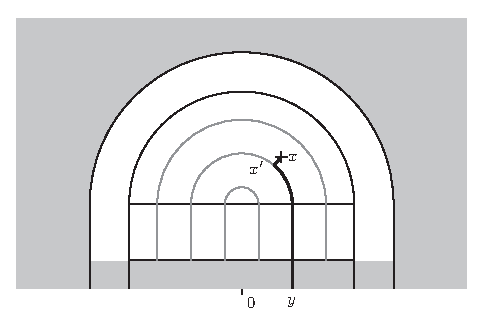
\includegraphics{Fig3}}
{\caption{The set $\{x \mid  f(x) = 0\}$ is shown in grey. The path
    in bold from an arbitrary $x \in \Omega$ to a point on $\partial \widetilde{M}_f$
    has length going to 0 as $\epsilon \to 0$}
  \label{fig:path}}
\end{figure}

\begin{table}[b]
\tabcolsep=0pt%
\TBL{\caption{This is table caption\label{tab1}}}
{\begin{fntable}
\begin{tabular*}{\textwidth}{@{\extracolsep{\fill}}lcccccc@{}}\toprule%
 & \multicolumn{3}{@{}c@{}}{\TCH{Element 1}}& \multicolumn{3}{@{}c@{}}{\TCH{Element 2\smash{\footnotemark[*]}}}
 \\\cmidrule{2-4}\cmidrule{5-7}%
\TCH{Projectile} & \TCH{Energy} & \TCH{$\sigma_{\mathit{calc}}$} & \TCH{$\sigma_{\mathit{expt}}$} &
\TCH{Energy} & \TCH{$\sigma_{\mathit{calc}}$} & \TCH{$\sigma_{\mathit{expt}}$} \\\midrule
\TCH{Element 3}&990 A &1168 &$1547\pm12$ &780 A &1166 &$1239\pm100$\\
{\TCH{Element 4}}&500 A &961 &$922\pm10$ &900 A &1268 &$1092\pm40$\\
\botrule
\end{tabular*}%
\footnotetext[*]{This is an example of table footnote}%
\end{fntable}}
\end{table}


For the volume of $\widetilde{M}_f$, taking $\rho = \epsilon$, the volume difference between
$\widetilde{M}_f$ and $M$ goes to 0 as $\epsilon \to 0$.
Indeed, using the fact that the chart $\psi$ is
a quasi-isometry, it is enough to show that the difference in volume between $S_f$ and
$\Omega \cup D$ goes to 0. Note that
$$
\mathop{\mbox{Vol}}(S_f)= \int_{\Omega \cup D}
\sqrt{1 + |\nabla f|^2} dx_1 \cdots dx_n\geq  \mathop{\mbox{Vol}}(\Omega \cup D).
$$
It follows from~\eqref{eq:nablafonA} and~\eqref{eq:nablafonB} that, on $\Omega$, the following holds:
$$|\nabla f|^2\leq1+\partial_2^2\omega^2=\epsilon^{-3}.$$
Similarly, it follows from~\eqref{eq:deffx} that on $D$, $$
|\nabla f|^2\leq c_5\Big(\frac{\partial_2^2}{\epsilon^2}+\partial_2^2\omega^2\Big)=c_5(\epsilon+\epsilon^{-3}),
$$
where $c_5$ is a positive constant.
It follows that
\begin{align*}
  |\mathop{\mbox{Vol}}(S_f) - \mathop{\mbox{Vol}}(\Omega \cup D)| &= \int_{\Omega \cup D}
  \sqrt{1 + |\nabla f|^2} dx_1 \cdots dx_n  - \mathop{\mbox{Vol}}(\Omega \cup D)\\
  &= \mathcal{O}(\epsilon^{n-3/2}),
\end{align*}
which goes to 0 for $n \geq 2$. Finally, it is clear that the curvatures of
$\partial \widetilde{M}_f$ do not change, as $M$ is kept fixed on some neighborhood
of the boundary due to the localisation of $f$ by the function $\gamma$, which vanishes near the boundary; see Figure~\ref{fig:path} and the definition~\eqref{eq:deffx} of $f$.
\end{proof}

\noindent Here is the sample for numbered list.
\begin{enumerate}
\item First item in the number list.
\item Second item in the number list.
\item Third item in the number list.
\end{enumerate}
Here is the sample for bulleted list.
\begin{itemize}
\item First item in the bullet list.
\item Second item in the bullet list.
\item Third item in the bullet list.
\end{itemize}
Here is the sample for description list.
\begin{description}
\item[First] item in the description list.
\item[Second] item in the description list.
\item[Third] item in the description list.
\end{description}

\section{Conclusion}

Some Conclusions here.

\begin{Backmatter}

\paragraph{Acknowledgments}
We are grateful for the technical assistance of A. Author.

\paragraph{Funding statement}
This research was supported by grants from the <funder-name><doi>(<award ID>); <funder-name><doi>(<award ID>).

\paragraph{Competing interests}
A statement about any financial, professional, contractual or personal relationships or situations that could be perceived to impact the presentation of the work --- or `None' if none exist

\paragraph{Data availability statement}
A statement about how to access data, code and other materials allowing users to understand, verify and replicate findings --- e.g. Replication data and code can be found in Harvard Dataverse: \url{https://doi.org/link}.

\paragraph{Ethical standards}
The research meets all ethical guidelines, including adherence to the legal requirements of the study country.

\paragraph{Author contributions}
A.A. and A.B.C. designed the study, abstracted the data wrote the first draft, and approved the final
version of the manuscript. A.R.E.J., M.R.L., K.L.S., and A.D.P. revised the manuscript and approved the final version.

\paragraph{Supplementary material}
State whether any supplementary material intended for publication has been provided with the submission.


\begin{thebibliography}{99}

\bibitem{Chavel}
I. Chavel, \emph{Eigenvalues in {R}iemannian geometry}. Pure and Applied Mathematics, 115, Academic Press, Inc., Orlando, FL, 1984.

\bibitem{CG18}
D. Cianci  and A. Girouard, \emph{Large spectral gaps for {S}teklov eigenvalues under volume 	constraints and under localized conformal deformations}. Ann. Global Anal. Geom. \textbf{54}(2018),  529--539. \doi{10.1007/s10455-018-9612-6}
	

\bibitem{CoursColboisMtl}
B. Colbois, \emph{The spectrum of the {L}aplacian: a geometric approach}. In: Geometric and computational spectral theory, Contemp. Math., 700, Amer. Math. Soc., Providence, RI, 2017, pp.~1--40. \doi{10.1090/conm/700/14181}

\bibitem{CESG17}
B. Colbois, A.  El Soufi,  and A. Girouard, \emph{Compact manifolds with fixed boundary and large {S}teklov eigenvalues}. Proc. Amer. Math. Soc. \textbf{147}(2019),  3813--3827. \doi{10.1090/proc/14426}


\bibitem{CGG17}
B. Colbois, A. Girouard,   and K. Gittins, \emph{Steklov eigenvalues of submanifolds with prescribed boundary in {E}uclidean space}. J. Geom. Anal. \textbf{29}(2019),  1811--1834. \doi{10.1007/s12220-018-0063-x}

\bibitem{CGH18}
B. Colbois, A. Girouard,   and A. Hassennezhad, \emph{The {S}teklov and {L}aplacian spectra of {R}iemannian manifolds with boundary}. 2018. \href{http://arxiv.org/abs/1810.00711}{\nolinkurl{arxiv:1810.00711}}


\bibitem{GPPS}
A. Girouard, L. Parnovski, I. Polterovich,	 and D. A. Sher, \emph{The {S}teklov spectrum of surfaces: asymptotics and invariants}. Math. Proc. Cambridge Philos. Soc. \textbf{157}(2014), 379--389. \doi{10.1017/S030500411400036X}


\bibitem{GP10}
A. Girouard  and I. Polterovich, \emph{On the {H}ersch--{P}ayne--{S}chiffer inequalities for {S}teklov eigenvalues}. Functional Analysis and its Applications \textbf{44}(2010), 106--117.


\bibitem{GP17}
A. Girouard  and I. Polterovich, \emph{Spectral geometry of the {S}teklov problem}. J. Spectr. Theory
\textbf{7}(2017), 321--359. \doi{10.4171/JST/164}

\bibitem{Hi76}
M. W. Hirsch, \emph{Differential topology}. Graduate Texts in Mathematics,  33, Springer-Verlag, New York-Heidelberg, 1976.

\bibitem{Kar15}
M. Karpukhin, \emph{Bounds between {L}aplace and {S}teklov eigenvalues on	nonnegatively curved manifolds}. Electron. Res. Announc. Math. Sci. \textbf{24}(2017),  100--109. \doi{10.3934/era.2017.24.011}

\bibitem{legacy}
N. Kuznetsov, T. Kulczycki, M. Kwa\'snicki, A. Nazarov,   S. Poborchi, I. Polterovich,  and B. Siudeja, \emph{The legacy of {V}ladimir {A}ndreevich {S}teklov}. Notices Amer. Math. Soc. \textbf{61}(2014), 9--22. \doi{10.1090/noti1073}

\bibitem{LeeUhlmann}
J. M. Lee  and G. Uhlmann, \emph{Determining anisotropic real-analytic conductivities by boundary measurements}. Comm. Pure Appl. Math. \textbf{42}(1989), 1097--1112, \doi{10.1002/cpa.3160420804}

\bibitem{PS16}
L. Provenzano  and J. Stubbe, \emph{Weyl-type bounds for {S}teklov eigenvalues}. J. Spectr. Theory \textbf{9}(2019), 349--377. \doi{10.4171/JST/250}

\bibitem{shamma}
S. E.	Shamma, \emph{Asymptotic behavior of {S}tekloff eigenvalues and	eigenfunctions}. SIAM J. Appl. Math. \textbf{20}(1971), 482--490. \doi{10.1137/0120050}

\bibitem{WX09}
Q. Wang and C. Xia, \emph{Sharp bounds for the first non-zero {S}tekloff eigenvalues}. J. Funct. Anal. \textbf{257}(2009), 2635--2644.	\doi{10.1016/j.jfa.2009.06.008}

\end{thebibliography}

\end{Backmatter}

\end{document}
